% Observer/Estimator
% Author: Dominik Haumann
\documentclass[a4paper,11pt]{article}
\usepackage[utf8x]{inputenc} % utf8 encoding

\usepackage{amsmath} % nice math symbols
\usepackage{bm} % bold math
\usepackage{color} % change text color        

\usepackage{tikz}

\usetikzlibrary{matrix} % for block alignment
\usetikzlibrary{arrows} % for arrow heads
\usetikzlibrary{calc} % for manimulation of coordinates

% TikZ styles for drawing
\tikzstyle{block} = [draw,rectangle,thick,minimum height=2em,minimum width=2em]
\tikzstyle{sum} = [draw,circle,inner sep=0mm,minimum size=2mm]
\tikzstyle{connector} = [->,thick]
\tikzstyle{line} = [thick]
\tikzstyle{branch} = [circle,inner sep=0pt,minimum size=1mm,fill=black,draw=black]
\tikzstyle{guide} = []
\tikzstyle{snakeline} = [connector, decorate, decoration={pre length=0.2cm,
                         post length=0.2cm, snake, amplitude=.4mm,
                         segment length=2mm},thick, magenta, ->]

\renewcommand{\vec}[1]{\ensuremath{\boldsymbol{#1}}} % bold vectors
\def \myneq {\skew{-2}\not =} % \neq alone skews the dash

\usepackage{minted}
\usepackage{mathtools}
\usetikzlibrary{positioning, calc}
\usepackage{subcaption}
\usepackage{caption}
\usepackage{graphicx}

\usepackage{geometry}
\geometry{%
letterpaper, % a4paper
left=   40 mm,
right=  40 mm,
top=    15 mm,
bottom= 20 mm,
}



\begin{document}


\begin{figure}
    \centering
    \begin{subfigure}[b]{0.49\textwidth}
    	\resizebox{\linewidth}{!}{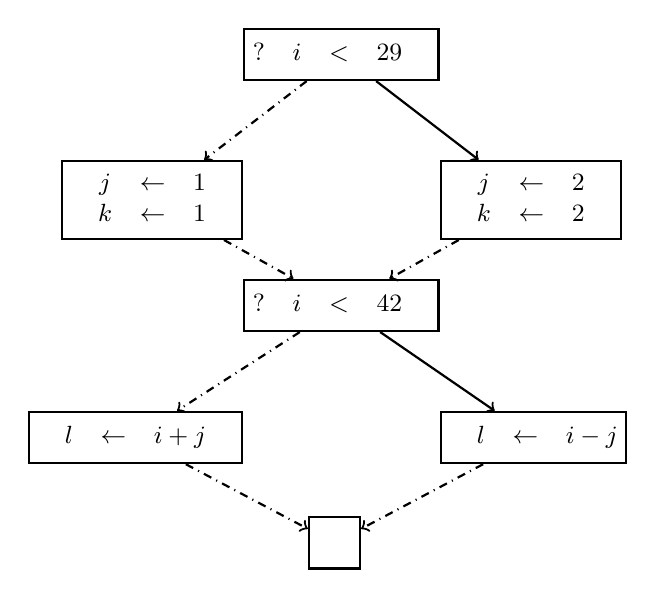
\begin{tikzpicture}
	\small
	  \node[block] (base) {$\begin{matrix*}
			? & i &<& 29 &\\
		  \end{matrix*}$
	   }; 
	  
	  \node[block, below left = 1cm and 0cm of base] (neg1) {
	  	$\begin{matrix*}
	  		&j &\gets& 1 &\\
	  		&k &\gets& 1 &
	  	\end{matrix*}$
	  }; 
	  
	  \node[block, below right = 1cm and 0cm of base] (pos1) {
		$\begin{matrix*}
			&j &\gets& 2& \\
			&k &\gets& 2&
		\end{matrix*}$
	  }; \&

	  \node[block, below = of {$(pos1)!0.5!(neg1)$}] (merge1) 		  			  {
	  $\begin{matrix*}
	  ? & i &<& 42 &\\
	  \end{matrix*}$
	  }; \&


	  \node[block, below left = 1cm and 0cm of merge1] (neg2) {
	  $\begin{matrix*}
	  &l &\gets& i + j &\\
	  \end{matrix*}$
	   
	  }; 
	  
	  \node[block, below right = 1cm and 0cm of merge1] (pos2) {
		$\begin{matrix*}
			&l &\gets& i - j \\
		\end{matrix*}$
		}; 
	  

	  \node[block, below = of {$(pos2)!0.5!(neg2)$}] (merge2) 		  			  {
	  $\begin{matrix*}

	  \end{matrix*}$
	  };

	% now link the nodes

	\draw [connector] (base) --  (pos1);
	\draw [dash dot, connector] (base) --  (neg1);
	\draw [dash dot, connector] (pos1) -- (merge1);
	\draw [dash dot, connector] (neg1) -- (merge1);
	\draw [connector] (merge1) -- (pos2);
	\draw [dash dot, connector] (merge1) -- (neg2);
	\draw [dash dot, connector] (pos2) -- (merge2);
	\draw [dash dot, connector] (neg2) -- (merge2);


  \end{tikzpicture}}
	    \caption{A gull}
	    \label{fig:gull}
	\end{subfigure}
    \begin{subfigure}[b]{0.49\textwidth}
    	\resizebox{\linewidth}{!}{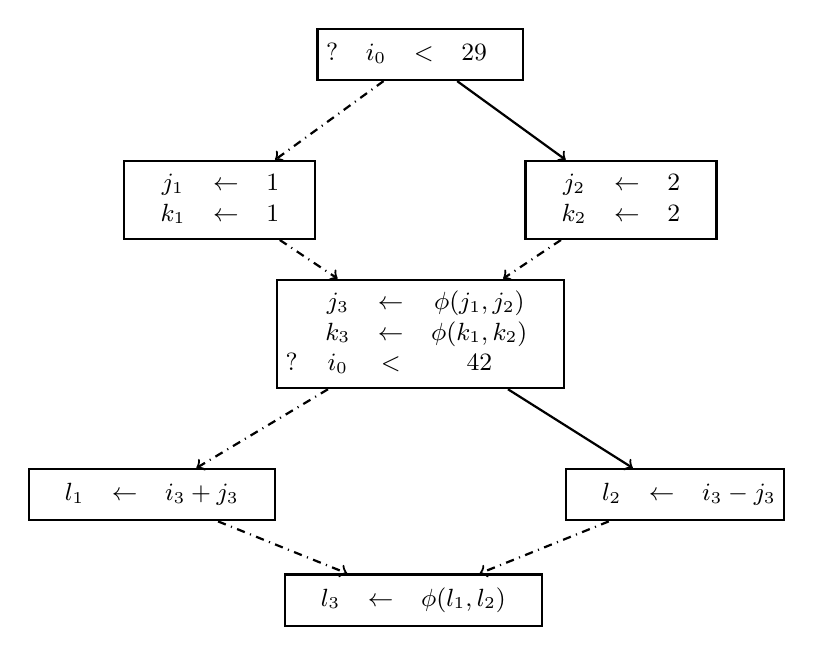
\begin{tikzpicture}
\small
  \node[block] (base) {$\begin{matrix*}
		? & i_0 &<& 29 &\\
	  \end{matrix*}$
   }; 
  
  \node[block, below left = 1cm and 0cm of base] (neg1) {
  	$\begin{matrix*}
  		&j_1 &\gets& 1 &\\
  		&k_1 &\gets& 1 &
  	\end{matrix*}$
  }; 
  
  \node[block, below right = 1cm and 0cm of base] (pos1) {
	$\begin{matrix*}
		&j_2 &\gets& 2& \\
		&k_2 &\gets& 2&
	\end{matrix*}$
  }; \&

  \node[block, below = of {$(pos1)!0.5!(neg1)$}] (merge1) 		  {
  	$\begin{matrix*}
  		&j_3 &\gets& \phi(j_1, j_2)& \\
  		&k_3 &\gets& \phi(k_1, k_2)& \\
  		? & i_0 &<& 42 &\\
  	\end{matrix*}$
  }; \&


  \node[block, below left = 1cm and 0cm of merge1] (neg2) {
  	$\begin{matrix*}
  		&l_1 &\gets& i_3 + j_3 &\\
  	\end{matrix*}$
   
  }; 
  
  \node[block, below right = 1cm and 0cm of merge1] (pos2) {
	$\begin{matrix*}
		&l_2 &\gets& i_3 - j_3 \\
	\end{matrix*}$
	}; 
  

  \node[block, below = of {$(pos2)!0.5!(neg2)$}] (merge2) 		  {
  	$\begin{matrix*}
		&l_3 &\gets& \phi(l_1, l_2)& \\
  	\end{matrix*}$
  };

% now link the nodes

\draw [connector] (base) --  (pos1);
\draw [dash dot, connector] (base) --  (neg1);
\draw [dash dot, connector] (pos1) -- (merge1);
\draw [dash dot, connector] (neg1) -- (merge1);
\draw [connector] (merge1) -- (pos2);
\draw [dash dot, connector] (merge1) -- (neg2);
\draw [dash dot, connector] (pos2) -- (merge2);
\draw [dash dot, connector] (neg2) -- (merge2);
\end{tikzpicture}}
        \caption{A tiger}
        \label{fig:tiger}
    \end{subfigure}
\end{figure}

  
  
  

\end{document}